% Monthly-Notices_template.tex
%
% This is an adaptation of mnras_template.tex
% which is a LaTeX template for creating an MNRAS paper
%
% v3.0 released 14 May 2015
% (version numbers match those of mnras.cls)
%
% Copyright (C) Royal Astronomical Society 2015
% Authors:
% Keith T. Smith (Royal Astronomical Society)

% Change log
%
% v3.0 May 2015
%    Renamed to match the new package name
%    Version number matches mnras.cls
%    A few minor tweaks to wording
% v1.0 September 2013
%    Beta testing only - never publicly released
%    First version: a simple (ish) template for creating an MNRAS paper

%%%%%%%%%%%%%%%%%%%%%%%%%%%%%%%%%%%%%%%%%%%%%%%%%%
% Basic setup. Most papers should leave these options alone.
\documentclass[a4paper,fleqn,usenatbib]{mnras}

% MNRAS is set in Times font. If you don't have this installed (most LaTeX
% installations will be fine) or prefer the old Computer Modern fonts, comment
% out the following line
\usepackage{newtxtext,newtxmath}
% Depending on your LaTeX fonts installation, you might get better results with one of these:
%\usepackage{mathptmx}
%\usepackage{txfonts}

% Use vector fonts, so it zooms properly in on-screen viewing software
% Don't change these lines unless you know what you are doing
\usepackage[T1]{fontenc}
\usepackage{ae,aecompl}


%%%%% AUTHORS - PLACE YOUR OWN PACKAGES HERE %%%%%

% Only include extra packages if you really need them. Common packages are:
\usepackage{graphicx}	% Including figure files
\usepackage{amsmath}	% Advanced maths commands
\usepackage{amssymb}	% Extra maths symbols
\usepackage{listings}

%%%%%%%%%%%%%%%%%%%%%%%%%%%%%%%%%%%%%%%%%%%%%%%%%%

%%%%% AUTHORS - PLACE YOUR OWN COMMANDS HERE %%%%%

% Please keep new commands to a minimum, and use \newcommand not \def to avoid
% overwriting existing commands. Example:
%\newcommand{\pcm}{\,cm$^{-2}$}	% per cm-squared

%%%%%%%%%%%%%%%%%%%%%%%%%%%%%%%%%%%%%%%%%%%%%%%%%%

%%%%%%%%%%%%%%%%%%% TITLE PAGE %%%%%%%%%%%%%%%%%%%

% Short title which is used in the headers, and title of the paper.
% Enter the title of your project inside the {...} brackets
\title[PHY480 Project]{Title of PHY480 report}

% The list of authors, and the short list which is used in the headers.
% Enter your registration number twice in the next line
\author[160207219]{160207219
\\
Department of Physics \&\ Astronomy, University of Sheffield}

\date{\today}

% Enter the current year, for the copyright statements etc.
\pubyear{2020}

% Don't change these lines
\begin{document}
\label{firstpage}
\pagerange{\pageref{firstpage}--\pageref{lastpage}}
\maketitle

% Abstract of the paper
\begin{abstract}
This  \LaTeX\ document serves as a template for the PHY480 Semester~II report in the format of MNRAS (Monthly Notices of the Royal Astronomical Society). The report should have a short abstract, up to about 200 words long, which summarizes the contents of the report, briefly describing its aims, methods, and main results.
It should be a single paragraph, and no references should appear in the abstract.
\end{abstract}


%%%%%%%%%%%%%%%%%%%%%%%%%%%%%%%%%%%%%%%%%%%%%%%%%%

%%%%%%%%%%%%%%%%% BODY OF PAPER %%%%%%%%%%%%%%%%%%


%This is a simple template for authors to write new MNRAS papers.
%See \texttt{mnras\_sample.tex} for a more complex example, and \texttt{mnras\_guide.tex} for a full user guide.

% body of paper here - Use proper section commands
% References should be done using the \cite, \ref, and \label commands

\section{Introduction}
\label{sec:introduction}

A key issue regarding modern day survey astronomy is the sheer amount of data available. The first step given any survey imagery is to determine which objects are of interest, and which are not. Previously this would be a very time consuming process of manual selection. With the advent of machine learning, a very real possibility of using a computer to perform this task arose. 

Historically a need existed to classify astronomical object, from distinguishing between types of stars\cite{HarvardClassification} to different types of nebulae\cite{Nebulae} and later galaxies\cite{Hubble}. This process was usually very labor intensive and involved the time of many a grad student. That changed in the latter part of the 20th century. Starting with applying the AutoClass algorithm to the IRAS catalogue in 1988[cite here], astronomers started using computers to solve this classification problem using machines.

Early methods for this involved selecting features manually and separating the feature-selected variables into classes. This however, was still quite labor-intensive and did not solve the fundamental problem which was human bias. Human bias exists within these kinds of methods because the features selected are often based on the understanding of the researchers themselves. Therefore any feature selected may be the tainted by the human selection of variables. An example of this was \cite{Abraham2000}, where they extracted features of galaxies which were based on their understanding---the features were early/late-type galaxies based on the Hubble sequence, and the strength of the central bar. While this report does not seek to discredit that paper, one should have a certain expectation that the results from this would then correspond to the Hubble 'tuning-fork' diagram due to the parameters selected---which it does. 

Next in the development of this field was the advent of PCA (principle component analysis) and SVM (support vector machine)---a lengthier discussion may be found in my Semester 1 Report. PCA enables feature selection that is blind to the researchers. This is because PCA essentially selects the principle components, which are linear combinations of the input features, and orders these principle components in order of variance (which can also be understood as information density). With this, one only needs to select as many principle components as one has the computing power to handle. This gives an objective way of both selecting features and dimension reduction. Using these principle components, it is possible to apply SVM to this now dimension-reduced dataset to classify the data if it is linearly separable. \cite{SVM} However, there are still some shortcomings with this method. Most importantly, SVM is only effective on linearly separable data, and real life data often is not. Therefore, more sophisticated methods such as the 'kernal-trick' \cite{kernaltrick} may be used to try and separate the data. However even with these methods to extend the applicability of SVM, it remains ineffective on some datasets. There are other classification algorithms such as logistic regression, but they continue to lack in classifying all datasets generally \cite{UniversalApproximationTheorem}. Another downfall is with PCA. Due to the nature of dimension reduction, some data must necessarily be discarded. Even though the PCA algorithm guarantees that the minimum amount of data will be discarded, some is discarded nonetheless. If one's computing power allows, it is clearly superior to not discard any data at all. 

The next step in this field happened relatively recently---within the last 5 years---and is mainly due to advances in hardware as well as breakthroughs in computer science. The use of a neural network has been discussed for some time before this [cite here], in fact a SVM classifier can be seen as a prototype of neural networks. However, for a long time, deeper neural networks were hampered by a lack of ability to train them effectively due to convergence issues with optimisers.[cite here] When this issue was solved, the field of machine learning was also aided by the exponential growth of processor speed (viz. Moore's Law), which allowed more complex (deep) neural networks to be designed and trained. However, this field is still lacking the push to prominence that the field of computer vision has today. 

That final push came in two forms: the unstable-gradient problem (also known as the the vanishing-gradient problem in certain instances, further discussion in Theory section below) was solved using further backpropogation (explained below) because hardware advances allowed this; and a shift of activation function because sigmoid functions sometimes cause a saturation in the final hidden layer \cite{ReLu}, this was remedied by using another activation function (ReLu function) that is ubiquitous in modern neural networks. This allowed deep convolutional neural networks to be used efficiently and thereby resulting in the rapid development of the field of Computer Vision. \cite{NeuralNetworksandDeepLearning}

The proximate cause for this project and hence report is that the Gravitational wave Optical Transient Observatory (GOTO) records a very large amount of data which needs to be classified. Because the amount of data is too large for any human to complete in any reasonable amount of time, machine learning was enlisted to solve this problem. 

The primary goal of this project is to create a classifier that could classify sources on the image into stars or galaxies. The secondary goal is to extend that classifier to determine between spiral and elliptical galaxies. 

This project approached this problem from a largely computer science perspective and therefore the techniques used stem from current techniques in computer science. 

\section{Theory}

Given that the project is a synthesis of the fields of survey astronomy and machine learning. Many of the terms and techniques used will be unfamiliar to astronomers who have not worked in the machine learning field. This section seeks to give an overview of the important parts which are necessary to understand this project. 
\subsection{Classifiers}

A classifier is defined as an algorithm which predicts the class of a datapoint. A classifier can be seen as approximating a mapping function $f$ from input variables $X$ to discrete output variable $y$. N.B. In machine learning, these variables may be matrix or tensor objects. A datapoint here simply means an instance of $X$ which the classifier needs to classify. [Towards data science https://towardsdatascience.com/machine-learning-classifiers-a5cc4e1b0623] Within this project, the datapoint is a single image cutout, and the output is a determination whether the image is a star or a galaxy. 

There are many classifiers in existence, broadly speaking there are placed into two categories: Lazy-learners, which only classify objects when a test object is required to be classified; and Eager-learners, which trains a model based on training-set data and then applies the model onto testing data. Artificial neural networks---which are used in this project---are eager-learners. Eager-learners have the advantage being very quick to apply to new data at the expense of a lengthy training process. 

Since simple classifiers are both classifiers in their own right, as well as acting as activation functions for more complex neural networks. 
\subsubsection{Logistic Regression/Sigmoid Activation Function}
The logistic regression algorithm attempts to split a dataset into two classes---a positive class represented by an output of 1, and a negative class represented by an output of 0. It uses the sigmoid function to do so.
\begin{equation}
h(X)=\sigma(Z) \textnormal{, where } \sigma(Z)=\frac{1}{1+e^{-Z}}
\end{equation}
h is a linear parameter which broadly speaking gives the probability that 'X' is in the positive class. 
From the above, it is clear that $\lim_{Z \to +\infty} \sigma(Z)=1$ and $\lim_{Z \to -\infty} \sigma(Z)=0$. This allows for the classification of X based on inputs to Z. 

Given that, as stated above, $X$ is a generalised variable representing all the features(variables) $\{x_1,x_2,x_3,...\}$ that are inputs to the sigmoid function. Therefore X is a (usually column) vector.

The formal definition of the sigmoid function in the context of logistic regression is 
\begin{equation}
	h_\theta(X)=\frac{1}{1+e^{-\theta^T X}}
\end{equation}
In Machine Learning the variable $\theta$ often denotes the weights applied to the generalised variable X to correctly predict the outcome. The $\theta^T$ in the exponent denotes the transpose of $\theta$ because $\theta$ is a column vector like X and so to multiply each weight by the appropriate variable, the transpose must be taken. N.B. An equivalent operation here is the dot product $\theta \cdot X$, however this is not usually used because it generalises poorly when multiple output $y$ are needed, i.e. when $y=\begin{bmatrix}
           y_{1} \\
           y_{2} \\
           y_{3} \\
           \vdots
         \end{bmatrix}$.

The precise details on how to train a logistic regression model is beyond the scope of this report, but broadly speaking, a $\theta$ is found such that it correctly predicts the class of any given X. 

Given that the sigmoid function is just a function that takes inputs from $-\infty$ to $+\infty$, and outputs a number between 0 and 1. In the case of logistic regression, this can be seen as a probability that the input belongs to either class, in more complex neural networks, this function can play the role of an activation function. An activation function is just a function which processes the inputs taken from one or multiple nodes and outputs it to some other node. The activation function itself resides within a node and has some node weight $\theta$ related to it. 

A sigmoid function was ubiquitous as an activation function before 2011 because it satisfies a few requirements that make such an activation function very useful. It is nonlinear, which enables a two layer network to be a universal approximator \cite{UniversalApproximationTheorem}, it is continuously differentiable which makes a gradient descent approach---a very common way of optimising a neural network---possible. However, it fails in some circumstances such as saturating the final hidden layer \cite{ReLu}. Therefore the field of machine learning has steadily shifted away from using sigmoid activation functions.

\subsubsection{Rectifier/Rectified Linear Unit}
A rectifier is just like a sigmoid function in that it serves as an activation function in a node. The rectifier function is defined
\begin{equation}
f(x)=\textnormal{max}(0,x)= \begin{cases} 0, & \mbox{for } x\leq0 \\ x, & \mbox{for } x>0 \end{cases}	
\end{equation}
This function was found in \cite{ReLu} and it quickly became the favoured choice of activation function for neural networks. In the same paper, it was shown that this function also satisfies the non-linearity requirement. This function is not differentiable everywhere though, its derivative at 0 is undefined. However there are two solutions to this: the analytic solution is to define the derivative as 0 or 1, since those are the values of the derivative of the function elsewhere---0 for $x<0$, 1 for $x>0$. If this derivative at 0 is defined, then the derivative for the function is continuous. The second solution is that in a practical context, a node would never reach 0, because of the nature of gradient descent, the local minima is never actually reached, there is always some small value above or below 0, therefore the issue of an undefined derivative is not reached. Finally, this activation function has the added benefit of having an infinite range: $(0,\infty]$, which increase the speed of convergence of a model.

\subsection{Neural Networks}
A neural network is a set of nodes (which include the aforementioned activation functions) arranged in a certain way. Pertinent to this project is the feedforward neural network (FNN) and the convolutional neural network (CNN) as those are the networks used.
\subsubsection{Feedforward Neural Networks}
A feedforward neural network (FNN) is a neural network only feeds data forward through the network, i.e. there are no loops. This is the most simple type of neural network but it is also the most versatile. Because the inputs can be any type of numerical data, of any dimension, the neural network can approximate anything (Universal Approximation Theorem) \cite{UniversalApproximationTheorem}. Formerly, an FNN may only have 1 hidden layer which is due to both problems with training a neural network with anything more than 1 hidden layer (backpropagation \cite{Backpropagation}), but also due to nomenclature: anything with more than 1 HL is called a deep feedforward neural network. With the advent of much more powerful hardware and also techniques to effectively train multi-layered neural networks, these 'deep' feedforward neural networks replaced single-layered neural networks in almost all applications. Thence, all of these neural networks were generically termed 'Feedfoward Neural Networks'.  [Not sure which parts can be cited, but probably find some recent online textbook somewhere]

[Insert diagram of generic FNN]

\subsubsection{Convolutional Neural Networks}
A convolutional neural network (CNN), strictly speaking, can be thought of as a type of FNN due to it not having any recurring loops. However, in practice it is generally thought of as distinct due to it having vastly different node behaviour. 

A CNN, like its name suggests, is a neural network which has nodes which perform convolutional operations. Convolution is most often approached in physics in terms of a signal being convolved with a background. This is essentially the same operation that a convolutional node performs. A convolutional filter is applied to an image, this consists of a kernel which describes the function---which is almost always a linear shape---that passes over the original image and passing the result into a new image. 

[Find picture of convolution]

A CNN has 3 types of layers: convolution layers, pooling layers, and a fully connected layer. A convolution layer performs a convolutional operation as described above. It has 4 key parameters: kernel, stride length, layer size, and activation function. The kernel describes the kernel which is passed over the incoming image, the key parameter of the kernel is the size---kernels are usually squares of 3x3, 5x5, or 7x7 size, with the size determining how many neighbouring pixels the filter wants to take into account. The stride length is how many pixels the filter jumps over before the next filter. The layer size is how many convolutional filters are passed over the incoming image. Because each nodes has different initial conditions, this represents the trainable part of the network. Finally, the activation function determines what value is outputted to any particular pixel. In a modern CNN it is usually ReLU due to it working better with sparse models. \cite{CNNSparse}

A pooling layer can be thought of as a specific type of convolutional layer in that the kernel is a flat one. Its main purpose is to reduce the dimension of the incoming image. 

[Insert pooling layer image]

There are two types of pooling layers: average pooling and max pooling. An average pooling layer inputs the average value of the pixels within the pooling filter and outputs them to the next image. A max pooling layer does essentially the same but with the maximum value of the pixels rather than the average value. This achieves the same amount of dimensionality reduction except the max pooling layer achieves noise suppression by discarding the noisy activations. The max pooling layer is therefore said to be superior to the average pooling layer. [Maybe cite tds https://towardsdatascience.com/a-comprehensive-guide-to-convolutional-neural-networks-the-eli5-way-3bd2b1164a53]. 

A fully connected layer is simply a layer from an FNN used to gather the results of the convolutional and pooling layers and output to a visible layer, of which the results can be used. In binary classification cases a binary activation function such as sigmoid, ReLU, or tanh can be used, while in multiple-class classification problem a function like softmax should be used instead. [cite softmax]

A key advantage for CNN with dealing with image data is the ability to take into account nearby pixels. Because the inputs to a FNN are essentially flattened vectors: $X=\begin{bmatrix}
           x_{1} \\
           x_{2} \\
           x_{3} \\
           \vdots
         \end{bmatrix}$, the elements in the vector---$x_1$ and $x_2$ for example are independent. This does not allow a pixel which is nearby to influence a neighbours' node, which is unsatisfactory in machine vision because a network built that way does not recognise 'edges' or 'sides' or any feature which is visually important.

\subsection{Optimisation algorithms}
In order for a neural network to be of any use to anyone it must be trained. Training is a process where the weights of the neural network are modified to better predict the desired outcome. The broad idea behind optimisation of a neural network is that one is trying to minimise some loss function. Given that the problem is a minimisation problem, it would make sense to use some kind of algorithm which takes into account the gradient of the hypersurface that the optimiser is attempting to optimise over because it is known that at local minima the gradient of the surface is 0. 

In a general form, the equation for gradient descent is 
\begin{equation}
\theta_{n+1}=\theta_{n}-\alpha\nabla J(\theta)	
\end{equation}
where $\theta$ is a general set of weights applied at any particular node. $\theta_{n}$ is the set of weights before updating while $\theta_{n+1}$ is that after updating. $\alpha$ is a variable called the learning rate, which controls how 'far' in any one direction one update moves the weights on the hypersurface. $\nabla J$ is the key term here as this is the gradient of the cost(loss) function over all variables which ensures all the weights for the variables are updated in the same pass. [probably cite the Stanford course]

\subsubsection{Stochastic Gradient Descent}
Stochastic Gradient Descent (SGD) is an algorithm which chooses a random datapoint within the whole dataset to perform the gradient descent algorithm. This was developed due to the need to train larger and larger datasets. Larger datasets present a challenge due to the longer time it takes to calculate losses through the entire dataset, at some point large datasets present a hardware constraint of not having enough RAM to store the entire dataset in memory which makes gradient descent through the whole dataset unworkable. 

SGD solves this by updating the weights after a single datapoint. This allows the weights to converge much quicker than in normal gradient descent. However, because each datapoint updates the gradient this introduces a lot of noise which cannot be removed. A modern compromise is to use mini-batches---updating the weights after every few 10s or 100s of datapoints. \cite{SGD}

\subsubsection{Momentum}
A modern advance to the gradient descent algorithm uses a concept called momentum. The full mathematical treatment of momentum is beyond the scope of this report, but a general explanation of the concept will be given. \cite{Momentum} The general concept of momentum is the addition of a variable $v$, representing the momentum of the descending 'particle'. The updating equations are changed to 
\begin{equation}
\begin{cases} v_{n+1}=\eta v_{n}-\alpha\nabla J(\theta)  \\ \theta_{n+1}=\theta_{n}+v_{n+1}\end{cases}
\end{equation}
with $v$ being the new momentum parameter and $\eta$ being a new decaying hyper-parameter. This has the effect of both accelerating convergence due to the momentum term accumulating a large value from repeated updates in the same direction; and the effect of smoothing out noise because local fluctuations in gradient get smoothed over by the overriding momentum term.

A variant of the momentum approach is the Nesterov Accelerated Gradient (NAG). The principle is essentially the same except the algorithm calculates the momentum using past values i.e. $v_{n}$ and $v_{n-1}$ in lieu of $v_{n+1}$ and $v_{n}$ respectively as well a slightly modifying the gradient calculation. This method has a key benefit of being able to 'slow down' the momentum before it reaches the minimum of the hyperplane thereby reducing the possibility of 'overshooting'.

\subsubsection{Modern Optimisers}
\label{section:modern optimizers}
Modern optimisers tend to use an adaptive learning rate.

[liberally get citations from here https://ruder.io/optimizing-gradient-descent/index.html]

 The learning rate $\alpha$ as described above in the aforementioned optimisers are constants. However it is often advantageous for the learning rate to change with respect to the parameters.
 
 The first modern optimiser in this regard is Adagrad (for 'adaptive gradient') published in 2011. \cite{AdaGrad} This implementation adds the adaptive gradient using a multiplicative term in the denominator that sums the squares of previous gradients. This method allows the learning rate to be greater in the beginning of training where, presumably, the parameters are further from the minimum; and decreasing as the minimum is approached. However, a downside to this method is the possibility that the accumulated terms decrease the learning rate so much as to have slowed the learning too much before reaching the minimum. Subsequent developments have solved this issue. 
 
 Adadelta is a modification on the Adagrad algorithm in which it truncates the accumulation term at some length. This prevents the eventual suppression of the learning rate to 0. \cite{AdaDelta}
 
 Adam (for 'Adaptive Moment Estimation') is an algorithm which is a development from Adadelta and another algorithm called RMSprop, which remains unpublished as of the time of writing. The Adam stores not only a average of the squared terms of past gradients---in Adam this is an exponential decay rather than a truncation, it also stores an average of past gradients. These are then used to update parameters similar to the above methods. \cite{Adam} Adam has become the dominant optimiser for neural networks within computer vision and natural language processing due to the result being favourable in comparison to other optimisers. 
 
 However, adaptive learning rate optimisers have the downside of not converging in certain circumstances. The details reason can be found here \cite{ObjectAMSGrad} and \cite{translateAMSGrad}. In 2018, \cite{AMSGrad} has modified the Adam algorithm where instead of using an exponentially decaying average, it uses the maximum value of past gradients to determine the learning rate and the momentum. This algorithm is called AMSGrad and the authors have included a proof of convergence that Adam lacks. This algorithm outperforms Adam on small datasets while shows similar or worse performance on other datasets. Since this algorithm is very new, it is yet to be determined if this algorithm is superior to Adam.
 
 
 \section{Method}
This section describes the method from which a functional neural network is yielded from the initial GOTO images.
\subsection{Cutout Algorithm}
The initial .fits files from GOTO are 6132x8176 pixels in size, and to prepare the images for training in a neural network, some preprocessing of the data is needed. 

A cutout algorithm was written for this. Since the images provided have already been processed, the science layer within the .fits file is assumed to be the true pixel intensity values and will be worked with directly. The values are directly extracted with to a data array (ndarray from numpy package).

\subsubsection{Source Detection}
The first step in the data processing is to perform source detection on the data. Source detection is performed using the  \texttt{detect\_sources} function within the \texttt{photutils} package. This function requires data, threshold, number of pixels and the filter kernel. The filter kernel is a smoothing algorithm that smoothes the incoming data by passing it through a kernel. In this case, the kernel is defined to be to cause the signal to be smoothed to a full-width half-maximum of 3 pixels. This helps the detection algorithm detect sources because the algorithm relies on contiguous pixels to detect sources and smearing out some light onto nearby pixels assists allows very small sources as well as artefacts to be detected.

The next input is the threshold which defines the threshold which the source will be detected. This threshold can be an absolute value for which the source must have a certain intensity to be detected. However, this fails to take into account the background of which the source lies on. Therefore, in the current implementation the background is taken into account by creating an estimated background using the \texttt{Background2D} function, also within the photutils package. This estimates a background of the image given some parameters and the data of the image. The key parameters is the box size, which determines across how many nearby pixels should the background be considered to be constructed over---in this case it is a 50x50 box which is a completely arbitrary number. Normally this box should be a divisor of both the total x and y pixels in the entire number due to edge effects that would be an issue if fractions of boxes are left at edges. Here, this is not an issue because the cutout algorithm---as shall be explained below---cuts out the edges of the image, so this is a non-factor. This background estimator uses a median estimator which estimates the background based on the median value rather than an average value. [cite photutils documentation] This is so because where a source would exist, these represent much higher values than the background values and an average would wrongly 'drag' up the results due to sources which patently are not part of the background. Finally the threshold which enters the source detection algorithm is defined as 10 times the estimated background at the point. This means that for a collection of pixels to be defined as a source, the source detection algorithm requires that the number of contiguous pixels which all have brightnesses greater than 10 times the estimated background be greater than the number of pixels defined in npixel. This is a tradeoff between computing time and number of sources detected. If this number was lower, the number of detected sources would increase exponentially, but much more noise would also be detected hence causing a drastic increase in script runtime. Further, because of further steps such as cross referencing all the sources, this increase leads to further slowdowns in efficiency which is undesirable. However, having a much higher number would discard dimmer and more diffuse sources. This is particularly problematic because galaxies, in particular spiral galaxies, are particular diffuse and dimmer galaxies would be discarded which would lead to a lack of any galaxies to classify. Therefore, 10 times the estimated background is the tradeoff made here. 

The number of contiguous pixels \texttt{npixels}, as mentioned above, is the number of contiguous pixels which all exceed the threshold. In the function \texttt{detect\_sources}, the default behaviour of this detection is that it considers all pixels which are side- or corner- connected to a pixel is considered contiguous---this is called 8-connected pixels and is left as-is in this implementation. 

The data which is inputted to the \texttt{npixels} is simply the raw data from the data array.

There is an additional step possible in this process which is to deblend the sources after detecting sources. Deblending is the process in which overlapping sources are distinguished from each other and listed separately. However, the current implement forsakes deblending for two reasons. First is that deblending is costly in terms of processing time---from experience adding the deblending step increases the processing time of the source detection part of the cutout algorithm by 5-10 time. While not an issue for the small scale of the current implementation, since the aspiration is for this to be applied to more data in larger applications of this algorithm, this processing time becomes significant and any savings in processing time is worth it. Second, because deblending deals with overlapping sources, this necessitates that the sources in question are actually overlapping. Therefore, any image-cutouts made from these sources are necessarily of both sources. Because of the implementation of this cutout algorithm also assigns classes (stars or galaxies), if two sources were overlapping and had one of each source, the result would be an entry of essentially the same overlapping source in each category which would present a problem in training the neural network eventually. 

The result of this is an object called a segmentation image. This object is an array with the same size as the data, but it marks pixels where a source is detected with a positive integer to indicate a source is detected.  This object is used in the \texttt{source\_properties} function and is called \texttt{segm} in the code. 

\subsubsection{Extracting Source Properties}
The data is then entered into the \texttt{source\_properties} function. This function takes primarily the data and the segmentation array as functions---it also takes World Coordinate System (wcs) information from the header which is required to reference the object's location in sky coordinates. This function outputs an object containing over 30 attributes containing the sources' properties. However, not all 30 attributes are relevant to this project---only 7 attributes are called: \texttt{xcentroid}, \texttt{ycentroid}, \texttt{sky\_centroid.ra}, \texttt{sky\_centroid.dec}, \texttt{elongation}, \lstinline{equivalent_radius}, \texttt{area}. 

Because the \texttt{source\_properties} function calculates the centroid and morphological features of sources [cite documentation], the defining characteristics of the sources detected are the x and y positions of each source's centroid in pixel-space which are represented by the \texttt{xcentroid} and \texttt{ycentroid} values. Because the wcs of the original image is inputted to this function, it does a conversion to the the sky coordinates (right ascension and declination) of the sources, which are the \texttt{sky\_centroid.ra}, \texttt{sky\_centroid.dec} values. 

The elongation value is defined as the ratio of lengths of the semi-major and semi-minor axes. This is equivalent to 1-ellipticity. This metric is useful for determining the whether the the object in question is a true sky object or an artefact. 

The area is a measure of the area of sky covered by the source, it has units of pixel-squared. Determining the area is useful because it allows some determination to be made regarding tendencies for either stars or galaxies to be larger on the sky. It is not used in the cutout algorithm, but is retained for further investigation. The equivalent radius is a derived quantity from area, it is the radius of a circle with the same area as the source, it has units of pixels. 


[Img of equiv radius vs elongation]

\subsubsection{Data Cleaning}
Before the sources can be cut out individually, it is important that as many non-objects i.e. artefacts, be excluded from the extraction. This is done by excluding any source with elongation above 10. This number is a rough estimate to exclude any source which is clearly an artefact [image of streaky lines], but not too low as to exclude highly elongated sources, especially galaxies. 

Another aspect of the data that needs to be cleaned is that by observation of the image, there is a smearing at the edges of the image which elongates sources. This yields subpar samples to train with and therefore it is beneficial to exclude these sources. Therefore all sources which have centroids within 400 pixels within the left and right edges and within 300 pixels within the top and bottom of the image are excluded. 300 or 400 pixels are arbitrary numbers but they are approximately 5\% of the total sizes in either dimension. This means that approximately 10\% of the sources in either dimension are excluded this way. 

\subsubsection{Database Matching}
Since labeled data is required for the training of the neural network, these labels must be acquired from a source external to the algorithm. In this project, labels are acquired from the SDSS database. 

To do this, a query within the \texttt{astroquery} package is made to the SDSS database. First, the algorithm requests all galaxies in the SDSS database with the constraints that: they are within the confines of the sky coordinates of the initial data image which is easily determined from the wcs data in the header of the .fits file, and that the galaxies are brighter than g-band magnitude 21. The magnitude threshold is an empirical determination based on number of sources returned---because the total number of detected sources from the image is determined beforehand, a magnitude which yields a similar number of sources should be correct. In practice, mag 20 yields too few and mag 22 yields too many sources, therefore a magnitude of 21 is chosen. 

This returns a list of sky coordinates which have galaxies matching the requirements. These sky coordinates are then matched against the sources detected using astropy's matching algorithm and all matches with a tolerance of 3 arcseconds are cut out. 

The cutout algorithm is astropy's \texttt{Cutout2D}. The algorithm makes cutouts of the images, each with a size of 40x40 pixels. Each cutout is stored in a .fits file which is stored in a folder which contains to galaxies. The algorithm then appends modified header data into each cutout which makes it easy to find the location of a cutout from the original image if the need arises. 

The same procedure is completed for stars instead of galaxies with the results being stored in a dedicated stars folder. 

This part of the algorithm appears to be highly multithreaded. Using an 8-core Intel core-i9 9900HK running at 3.6GHz, it takes approximately 45 seconds for the algorithm to cut out each original image while it takes a 4-core Intel core-i7 6920HQ running 2.9GHz around 95 seconds on average. While there are some overhead losses, the performance seems to almost double with a doubling of the cores.
\subsection{FNN}
The first step in making a neural network of any kind is to determine the network architecture. The network architecture is a description of the 'shape' of the neural network. The network architecture describes how many layers, and what type of layers exist between the input and output. It also describes the size of each layer---i.e. how many neuron/nodes a layer has. 

[insert simple FNN architecture description]

The building a network architecture is not an exact science and is usually highly empirical and depends on the dataset. Over the few years that FNNs have existed, there are a few guidelines which are found to work well. First, a FNN should have the minimum number of layers and nodes possible to solve a given problem to the desired degree. The reason for this is twofold---one should minimise the number of layers to train because each layer represents additional computational time which is required to train a neural network. (probably exponential, but im not sure, maybe find a cite?) Another reason is that larger neural networks are very prone to overfitting and hence lack generality to be applied to other datasets. The empirical rule here is that the number of trainable parameters in any given neural network should be smaller than the number of datapoints in the dataset the network is trained over. 

Second, FNNs layers should be built in decreasing size. The size of a layer can be thought of as the dimension the data has at that point. And so the reason this rule exists can be generally be explained as FNNs compressing highly dimensional data into a 1D output should be done sequentially because there is not much purpose in re-expanding data into a larger dimensional space because the data could already be expressed in a lower dimensional space. This means that nothing is gained from having a non-strictly decreasing size. 

Third, non-linearly separable data should be treated with at least 2 hidden layer FNNs with non-linear activation functions. The reason for having at least 2 hidden layers is due to the Universal Approximation Theorem [cite], however, because the UAT describes a mathematical optimal situation, often more than 2 layers are used, but this gives the lower bound on the number of layers necessary. The requirement for non-linear activation functions is because it can be shown [mathematical proof] that an infinite number of linear activation unit layers are required to provide the result of a single layered non-linear activation unit and that it is impossible to do better---i.e. mimic multi-layered non-linear activation functions. [maybe add analogy to taylor expansions, or maybe not]

The FNN used in this project largely has these rules in mind when built. The FNN architecture is shown in [Figure]. As seen, the architecture has size 64,32,16 feedforward layers in sequence with all activation functions being ReLU. This gives $64\times 32+32\times 16 +16\times 1 = 2576$ trainable parameters. This is lower than the total number of images used for training (5075 images). This network has 3 hidden layers which is generally thought to be a good number of hidden layers for a general FNN classifier. 

The way this FNN is trained is using a train-test split approach. This means that the total number of datapoints are split randomly into two groups, with one group being used to train the network while the other group being used to test the performance of the network. The two groups of data are kept separate to each other so the test dataset is thought to simulate unlabelled general datapoints which the neural network is applied to. In the current application the train/test split is 0.8/0.2, meaning 80\% of the data is used to train and 20\% of the data is used to test the neural network. 

Each training datapoint is first flattened from a 40$\times$40 matrix into a 1600$\times$1 vector and placed into an array with all the other datapoints. This is valid due to [some theorem]. The data is subsequently scaled using a standard scaler---this changes the range of the data using an algorithm that takes into account the standard deviation (variance) of the images. This is done because nearby objects are brighter than further objects, but the morphologies should be the same, therefore a bias should be avoided here. After preprocessing, the data is then used to train the data. 

[section about keras? or is that too specific]

After training, the trained model is first saved to file which enable it to be used by anyone who needs to use this and removes the need for everyone to train their own model. Then the model is applied to the testing data. The model takes in each datapoints vector and outputs a single value, which ranges from 0 to 1. This value represents the network's predicted probability of this specific datapoint being a star or a galaxy---a datapoint which the network is certain is a galaxy will output a 1, and 0 for points which it is certain to be a star. And, using a threshold of 0.5, a confusion matrix and various metrics of the network can be determined. 
\subsection{CNN}
Due to the unsatisfactory of the FNN approach, a CNN based approached is designed instead. It was hoped that because a CNN makes use of neighbouring relations, it is better suited to classifying images. 
\subsubsection{CNN from scratch}
Just like in the FNN approach, the first step in using a CNN is to make one. However, there is even less guidance on how to make a good CNN due to the novelty of the field. In general, the rules from FNN still apply because CNNs can be thought of as FNNs with convolutional layers instead of feedforward layers. But due to the additional of pooling layers, the whole situation is much more complex. 

For this purpose, a CNN has been constructed similar to the FNN above, but with pooling layers between the convolutional layers [Figure]. However, a key difference is in the data preprocessing. In the FNN model, each of the datapoints are a flattened vector and then normally scaled. However, in the CNN implementation, each datapoint is an unflattened matrix (array) with the data not scaled in any way. This lack of scaling is due to the understanding that since a CNN 'sees' morphological features such as edges and corners, it should not matter what the absolute brightness of the pixel is. 

[keras is pretty much plug and play, but is the relevant]

The data was stored in an 3D array (tensor, in linear algebra terms) which are the 2D arrays for each image stacked on each other. The rest of the method is the same. 
\subsubsection{CNN from studying MNIST}
Given that the CNN that was built from scratch did not provide the results that were desired, an alternative was sought. It was realised that the current problem of classifying stars and galaxies from cutouts is quite similar to a dataset ubiquitous to CNN courses which is the MNIST dataset. [cite the dataset] This dataset contains hand drawn numerals (0-9) which is encoded in single channel 28$\times$28 pixel files. This is very similar to the cutout images used in this project, which are also single channel, but are 40$\times$40 in size and have only two classes. 

There was a model found which claims to be 'the best' model for classifying the MNIST dataset. This was easily modified to apply to the current project. 

Of note in that model was that, where one would expect a pooling layer, there was a convolutional layer with stride length 2. It is not immediately obvious why that would yield better results, but it is speculated that since pooling layers represent only dimension reduction without allowing for any training on the inputs/outputs, this stride length increased convolutional layer allows for dimension reduction while also increasing the number of trainable parameters. This comes, however, at the expense of requiring more calculation time. This is not an issue so far, however, because training times are on the order of 2 hours on the current hardware and dataset. Larger datasets and different hardware may well require different considerations on tradeoffs. 

\subsubsection{Optimisers}
There are a variety of optimisers available for selection within the neural network package used. Because most modern implementations of neural neural networks use some kind of adaptive gradient, initially AdaDelta was chosen as the optimiser. However, the accuracy reached using AdaDelta was not as good expected, therefore the Adam optimiser was used instead. This yielded good results, but also would occasionally return meaningless results of 50\% accuracy---50\% accuracy means a classifier which does no better than random chance. The reason for this is probably due to the momentum aspect of Adam---i.e. it accumulates too much momentum and doesn't manage to stop in the minimum. However, the solution to this, as described in the above section \ref{section:modern optimizers}, a solution which was a modification to the Adam algorithm---AMSgrad was released in 2018. This modification is also implemented in the neural network packaged used hence it was directly used. The result is that the neural networks using Adam and AMSgrad all converge, and contrary to some preliminary findings, there was no appreciable decrease in performance (convergence time). 

The neural networks were trained for 1024 epochs, with a batch size of 32. This means that each batch includes 32 images and the whole dataset was 'run through' 1024 times for the duration of the training. 

\subsection{Data Augmentation}
One key areas that is discovered in the generation of cutout images is that vastly more stars than galaxy are present in the dataset. So far, because equal number of each class must be preserved, a majority of stars are discarded and not used for training. This seems unsatisfactory and wasteful, therefore data augmentation was performed on the images. Data augmentation is the process of artificially increasing the amount of data available to train with. The data augmentation performed on the galaxy images. Because galaxies on the sky can appear in any orientation, the galaxy images were rotated by 90,180,270 degrees to form 3 additional images, and each of these, including the original one was reflected along one axis to form a total of 8 times more galaxy images. Given that there are now 8 times as many galaxy images as before, 8 times as many stellar images may be used. Because there is a wealth of stellar images, the increased images may be taken directly, and hence are unique images. The results of training using data acquired from this process are detailed below.
\section{Results}
In discussing the results, there are a few ways to quantify the quality of the classifier. This should be balanced against the time it takes to train the neural network which is relevant especially as the time increases to the order of days. To determine the goodness of the classifier, one should use metrics to determine how well the classifier classifies. Here, since this is a binary classifier, there are a  number of well established metrics which can be used. 

A confusion matrix is a matrix which groups the results of the classification into whether they are classified correctly or not. In a binary classifier, the confusion matrix has the form $CM=\begin{bmatrix}
           TP & FP \\
           FN & TN \\
         \end{bmatrix}$ , where TP stands for 'True Positive', which is the number of correctly classified 'positive' datapoints---in this project, since the purpose is to find galaxies, galaxies will be assigned as 'positive' results, the opposite assignation can be done with no loss in validity and will result in a transposed version of the same matrix. TN stands for 'True Negative', which is the number of correctly classified 'negative' datapoints---here stars. FP are 'negative' datapoints which the classifiers misclassify as positive---a star which the classifier classifies as galaxies, and finally FN is the opposite---an image of a galaxy which is misclassified as a star. In general, a good classifier should have a high $\frac{tr(CM)}{\sum{CM}-tr(CM)}$, where $tr(CM)$ is the trace of the confusion matrix, and $\sum{CM}$ is the sum of all elements in the confusion matrix. In essence, this quantity is the ratio of correctly classified datapoints to incorrectly classified datapoints. From this, more metrics could be defined to better quantify the performance of the classifier. 
         
 One of the most common metrics used is accuracy. It is defined as 
 \begin{equation}
 	ACC=\frac{TP+TN}{P+N}
 \end{equation}
  where P is the total number of Positive datapoints in total, and N is the total number of Negative datapoints in total. This is very intuitive as this is simply the percentage of the total amount of correct classifications. NB: A corresponding metric called the error rate is simply 1-Accuracy. Accuracy as a metric is generally good enough for most general classification purposes. However, there are cases, such as unbalanced datasets or when the purity of the prediction is important, where other metrics are important. 
  
  Sensitivity (or recall or true positive rate) is defined as follows
  \begin{equation}
  SN=\frac{TP}{P}	
  \end{equation}
This metric shows the fraction of correctly classified positive datapoints in all positive datapoints. This metric is important when the positive dataset is very small, such as when looking at a rare signal in a large amount of noise. 

  Precision (or positive predictive value) is defined as follows
  \begin{equation}
  PREC=\frac{TP}{TP+FP}	
  \end{equation}
This metric shows the fraction of correctly classified positive datapoints in all datapoints predicted as positive. This metric is important when the purity of the positive classified dataset is important.

From these 3 metrics and the confusion matrix itself, a further refinement/development of classification metrics can be developed. Matthews Correlation Coefficient is a metric which takes into account both the positive and negative classification. [cite probably original paper] It is defined thus
\begin{equation}
MCC = \frac{TP\times TN - FP\times FN}{\sqrt{(TP+FP)(TP+FN)(TP+FP)(TN+FN)}}	
\end{equation}
The Matthews Correlation Coefficient ranges from -1 to 1, where a coefficient of 1 represents a perfect classifier while a coefficient of -1 represents a classifier which assigns positive classification to all negative values and vice versa. A coefficient of 0 represents a random classifier. This coefficient has its roots in statistical theory and is related to the phi coefficient which is in turn related to the chi-squared statistic. When the confusion matrix is seen as a 2x2 contingency table, the relation is as follows
\begin{equation}
|MCC| = \phi = \frac{\chi^2}{n}
\end{equation}
where n is the total number of items in the contingency table. 

The F-score is a score which only takes into consideration the positive classification. There are many F-scores, all of which are harmonic means of precision and sensitivity. [cite] It is defined as follows
\begin{equation}
F_\beta = \frac{(1+\beta^2)(PREC\cdot SN)}{\beta^2 \cdot PREC + SN}
\end{equation}
The most used F-score is the $F_1$ score. 
\begin{equation}
F_1 = \frac{2(PREC\cdot SN)}{PREC + SN}
\end{equation}
$F_1$ ranges from 0 to 1, where a score of 1 represents a classifier which classifies all positive datapoints as positive but no others. A score of 0 represents the classifier did not classify any positive datapoints as positive. As one can see, this metric only accounts for the positive classifications and neglect the negative classifications entirely. 

Therefore the $F_1$ score is more appropriate when only the positive class is important---in this project, if one were only to be interested in extracting only galaxies in the image, for example. The Matthews Correlation Coefficient is important when one requires correct classifications for both classes---in this project, if one is performing a statistical study of all the stars and galaxies in the field, for example. 

Below, the accuracy, $F_1$ score and the Matthew Correlation Coefficient will be tabulated below for the FNN model, the CNN model built from scratch, the CNN model from studying the MNIST model, the CNN model built from scratch with data augmented, and the CNN model from studying the MNIST model with data augmented. See Table \ref{table:results}.


\begin{table*}
 \begin{tabular}{c||c c c||} 
 \hline
  & Accuracy & $F_1$ Score & Matthews Correlation Coefficient \\ [0.5ex] 
 \hline\hline
 FNN model & 85.760\% & 85.668\% & 71.521\% \\ 
 \hline
 CNN model built from scratch & 91.760\% & 91.633\% & 83.519\% \\
 \hline
 CNN model from studying the MNIST model & 92.880\% & 92.477\% & 85.940\% \\
 \hline
  CNN model built from scratch with data augmented & 93.116\% & 93.043\% & 86.254\% \\
 \hline
 CNN model from studying the MNIST model with data augmented & 93.926\% & 93.798\% & 87.935\% \\
 \hline
\end{tabular}
\caption{Table of results gained from the 6 different configurations of models used. Accuracy $F_	1$ score and Matthews Correlation Coefficient given. \label{table:results}}
\end{table*}
[insert numbers later]
\section{Discussion}
These results indicate that the CNN models are clearly superior to the FNN models at classifying images, which is expected. However, models trained on augmented data seem to perform worse across the board in comparison to models not. This may be because the act of augmenting data does not actually increase the variance (amount of information in the images) in the galaxy images. Therefore, with the increase in total amount of data, the network is not expected to perform as well. However, the difference is not conclusively separated from statistical variance. However, using augmented data means increasing the amount of data trained by 8 times, which correspondingly increases training time. Therefore, augmenting one class of data to train is generally inadvisable. A better approach would be to assign different weighting to training each class which would enable the use of unbalanced datasets. However this would increase the complexity of the code somewhat. 

Another thing of note here is that the $F_1$ score and Matthews Correlation Coefficient seems to vary together in each dataset and model. This indicates that no one model is especially suited to extracting galaxies which is a speculative use for a model like this. 

The threshold for this model is set at 0.5. On deeper inspection, it is found that the model tends to yield very extreme results. [see inserted diagram] This means that moving the threshold would not be very useful in increasing the precision in detecting galaxies. This means that to improve this model, it is not as simple as moving the threshold. 

[insert diagram of probabilities] 

Ultimately, in the best case result, the model yields a classification accuracy of 95\% and a Matthews Correlation Coefficient in the region of 80\%. This is not good enough for doing catalogue classification as there are a sizeable portion of impurities in both classifications. However, this shows that neural networks currently are good to use as tool for performing a 'first-pass' approach towards new datasets because this weeds out a great majority of incorrect datapoints. If a purer sample is required, one simply has to select from the classes given by the classifier because the datasets after classification is much denser in the desired class. An practical example is that if one were to want to study galaxies, after classification by this neural network, one only has to select galaxies from the galaxy class in this neural network. This is much easier than selecting from the overall dataset because the dataset is much small here and also much closer to a pure sample so one has to examine a much smaller number of images to reach the desired number of samples. 

\subsection{Future Improvements}
A key source of possible improvement is adding more data to train the model. At the moment, there is no lack of data, since data the data required to train the model is simply images which is captured by GOTO, but also in the SDSS catalogues. The overlap of these datasets are quite large and so there is no lack of data here. 

A concern at large datasets, however, is a memory problem. Since computers have finite RAM, at large datasets, the size of the dataset would frequently exceed the RAM of a regular computer. The train-test split approach relies on loading the entire dataset into RAM before performing operations on it. This would not work if the dataset exceeds RAM size. In research applications, the hardware is usually either processing speed bound (CPU and GPU are limitation, while RAM is effectively unlimited), or memory bound (RAM is limited, while processing power is very high, usually by way of CPUs with very high core counts). In processor-bound applications, the train-test split is appropriate because RAM is faster than loading from disk and has the benefit of knowing what the entire dataset looks like beforehand and therefore allows for some preprocessing. In memory-bound applications however, the train-test split does not work and instead an alternative method must be sought. A popular method for image recognition is the dataloader approach. [cite] This approach only retrieves images which are needed for the specific training batch and therefore the memory requirements are much smaller, but has a trade off of requiring much more processing power as well as needing a fast storage medium. 

With respect to the network architecture, the exact architecture that is best for the dataset varies per dataset. It is highly unlikely that any of the architectures used in this project is the optimal one. To determine the best network architecture, either a manual approach is needed to tune the hyperparameters of the system. This frequently entails using a validation set data. Since, the MNIST model was used directly, this process was omitted but probably have yielded some improvement in performance. This process is highly time consuming as the model needs to be retrained over each iteration of the network architecture. Some very new packages such as Google's AutoML [cite], and the open source AutoKeras [cite] have this training functionality inbuilt. But due to package incompatibility issues which are unresolvable until a new patch is released, this path could not be explored, but in the future this may well be the way forward. 

[insert some numbers with literature to compare?]

\section{Conclusion}
This project proves the viability of using a neural network classify to assist in the work of survey astronomy. An example of how this neural network could be implemented is provided. In the future, it may be possible to completely automate the classification process in catalogues, but this is not possible at the current stage. This project also illustrates the challenges in this area frequently lie in issues yielding labeled data instead of the actual usage of that data. Once labeled data is created, extant computer science techniques are readily available to be applied to this data to create a classifier. 

\pagebreak




The report should focus on the work done during semester two. The report should be written so as to be understandable to a non-specialist physics graduate and should follow the standard structure of a scientific paper. 

The report should be self-contained in the sense that it should not be necessary to have to re-read your report from semester~I in order to understand what the project is about. The report should therefore begin with a good introduction that explains the context of the work that you have done for your project. It should explain what your project was about, what you intended to do, and why this is important / useful / interesting. This introduction should include the references that underpin the work. There will, therefore, be some overlap with the literature review from semester I.

The report will be assessed independently by your supervisor and another academic. The second academic will normally be the same one who assessed your report in semester~I. This means that he/she will be someone who works in the same general area as the project topic (e.g. high-energy physics), but will {\em not} be familiar with the details of the project. Do not assume that the assessor should remember things from your Semester~I report. The marks of the second assessor carry equal weight as those of your supervisor, and so it is important that you explain clearly the context of your project and discuss any specialist techniques that you have used in language that is comprehensible to a physicist who is not working in exactly the same research area.



The main criteria for assessment will be the coherence of the scientific argument, the quality of the results obtained and their analysis, and the level of understanding displayed. However, marks may be deducted for poor written English, which  includes spelling (remember to use the `spell check' facility on the word processor), syntax and punctuation. Allowance will be made for students whose first language is not English. You will also lose marks for poor scientific style concerning equations, references, figures, tables, etc. 

The two assessors will award you a mark out of 50 for your report. The 50 marks are broken down into two categories:
\begin{description}
% The argument of \item in a LaTeX description envirnment should normally come out in bold, 
% but it seems that you have to do this manually in the MNRAS package.
\item[\textbf{Content}] Aims and objectives, description of relevant theories / experimental techniques, quality of results obtained, interpretation and analysis of results.
 \textbf{(30 marks)}
\item[\textbf{Clarity and presentation}] Organisation and structure, conciseness, quality of language, clarity of presentation, references, quality and appropriateness of diagrams and figures.
 \textbf{(20 marks)}
\end{description}
The marks of the two assessors will be averaged, and will count as 50\% of the overall semester II mark. The other 50\% of the semester~II marks are awarded as follows:
\begin{description}
\item[\textbf{25\%}] Project attempt.
\item[\textbf{25\%}] Oral examination (a.k.a. the `\textit{viva}').
\end{description}
The overall semester~II mark counts as 75\% of the PHY480 module mark, with the other 25\% being your semester~I report. 

\textit{Special note for 2020.} The coronavirus pandemic makes the submission and assessment of lab-books impractical. You are therefore no longer required to submit your lab-book, and the 25 marks previously assigned for ``project attempt and lab-book'' will now be allocated entirely to the supervisor's project attempt mark.








\section{Preparation of the report}
The report should be written in appropriate scientific language. You should avoid the use of jargon, but if you do use jargon or acronyms, they should be defined before use.  

The project plan that you wrote for your semester I report should be attached verbatim as Appendix~\ref{App:project plan}. In the write up of your work in semester II, you should discuss how well you kept to the plan. If you departed significantly from the plan, you should explain why this was done.

\textit{Special guidance for 2020 reports}. This year, it is probable that many of you will have had to depart from your original plan due to the coronavirus pandemic. It is also possible that your project was affected by the industrial action. In these cases, please explain how your project was affected, and what revised plan you followed as a consequence. This statement should be included as Appendix~\ref{2020 special}. Please make a reference to this appendix when you discuss your project plan in the main body of your report. You can write as much as you like in the Appendix, as the appendices are not included in the word limit. 
If your project was not affected, please just write something like ``My project was not significantly affected either by the industrial action or the coronavirus'' in Appendix~\ref{2020 special}. Note that you might still have changed your plan even if there had been no industrial action or coronavirus. These changes to your plan should be discussed in your report, just as in all previous years.

 
The total length of the report should not exceed about 10,000 words, excluding the appendices. You can have as many words as you need for your appendices. A quick way to estimate the word count of a \LaTeX\ document is to create a PDF file, select and copy the relevant parts  of the report, and then paste into a word processor that has a word counting facility (e.g. WORD).

Some of you may wish to refer back to material from the preliminary work section of your first semester report. This is permitted, but you need to make sure that the semester II report is self-contained, as explained in Section~\ref{sec:introduction}. One option is to summarize the results from Semester~I in an Appendix called something like ``Summary of results from preliminary work in Semester~I'', and refer to this Appendix as needed within the main body of your report. If you include results from your Semester~I report, you \textit{must} make it clear that these results are from the previous report. For example, if you reproduce a data graph in the main body of your report, you must give a citation to your Semester~I report, such as \citep{semester 1 report}. The reports will be submitted through Turnitin, which will pick up the overlap with the previous report. Unless the origin of the material from the previous report is properly acknowledged, its re-use is considered plagiarism, as that material has already been assessed.

 The use of figures and tables can greatly improve the presentation of your project. For figures, the legends, annotations and axes labels, including units, must be clearly indicated. To include figures in a \LaTeX\ document, you first need to generate an image file (JPEG, PNG or PDF), and then use the {\tt includegraphics} command to include it in your document. Make sure that the axis labels are easily readable by ageing assessors with poor eyesight. Use the {\tt figure} environment and the {\tt caption} command to add a number and a caption to your figure. See the code for Figure \ref{fig:eclipse} for an example. There is no limit to the number of figures you can include. 
Figures taken or adapted from published sources should be appropriately referenced, as in Fig.~\ref{fig:eclipse}.

All equations should be numbered, as in eqn~\ref{E=mc2}:
\begin{equation}
\label{E=mc2}
E = mc^2 \, .
\end{equation}


% In two-column mode, this environment will change to single-column
% format so that long equations can be displayed. Use
% sparingly.
%\begin{widetext}
% put long equation here
%\end{widetext}

The report must be submitted according to strict Journal formatting rules. See Section~\ref{sec:format}.

\begin{figure}
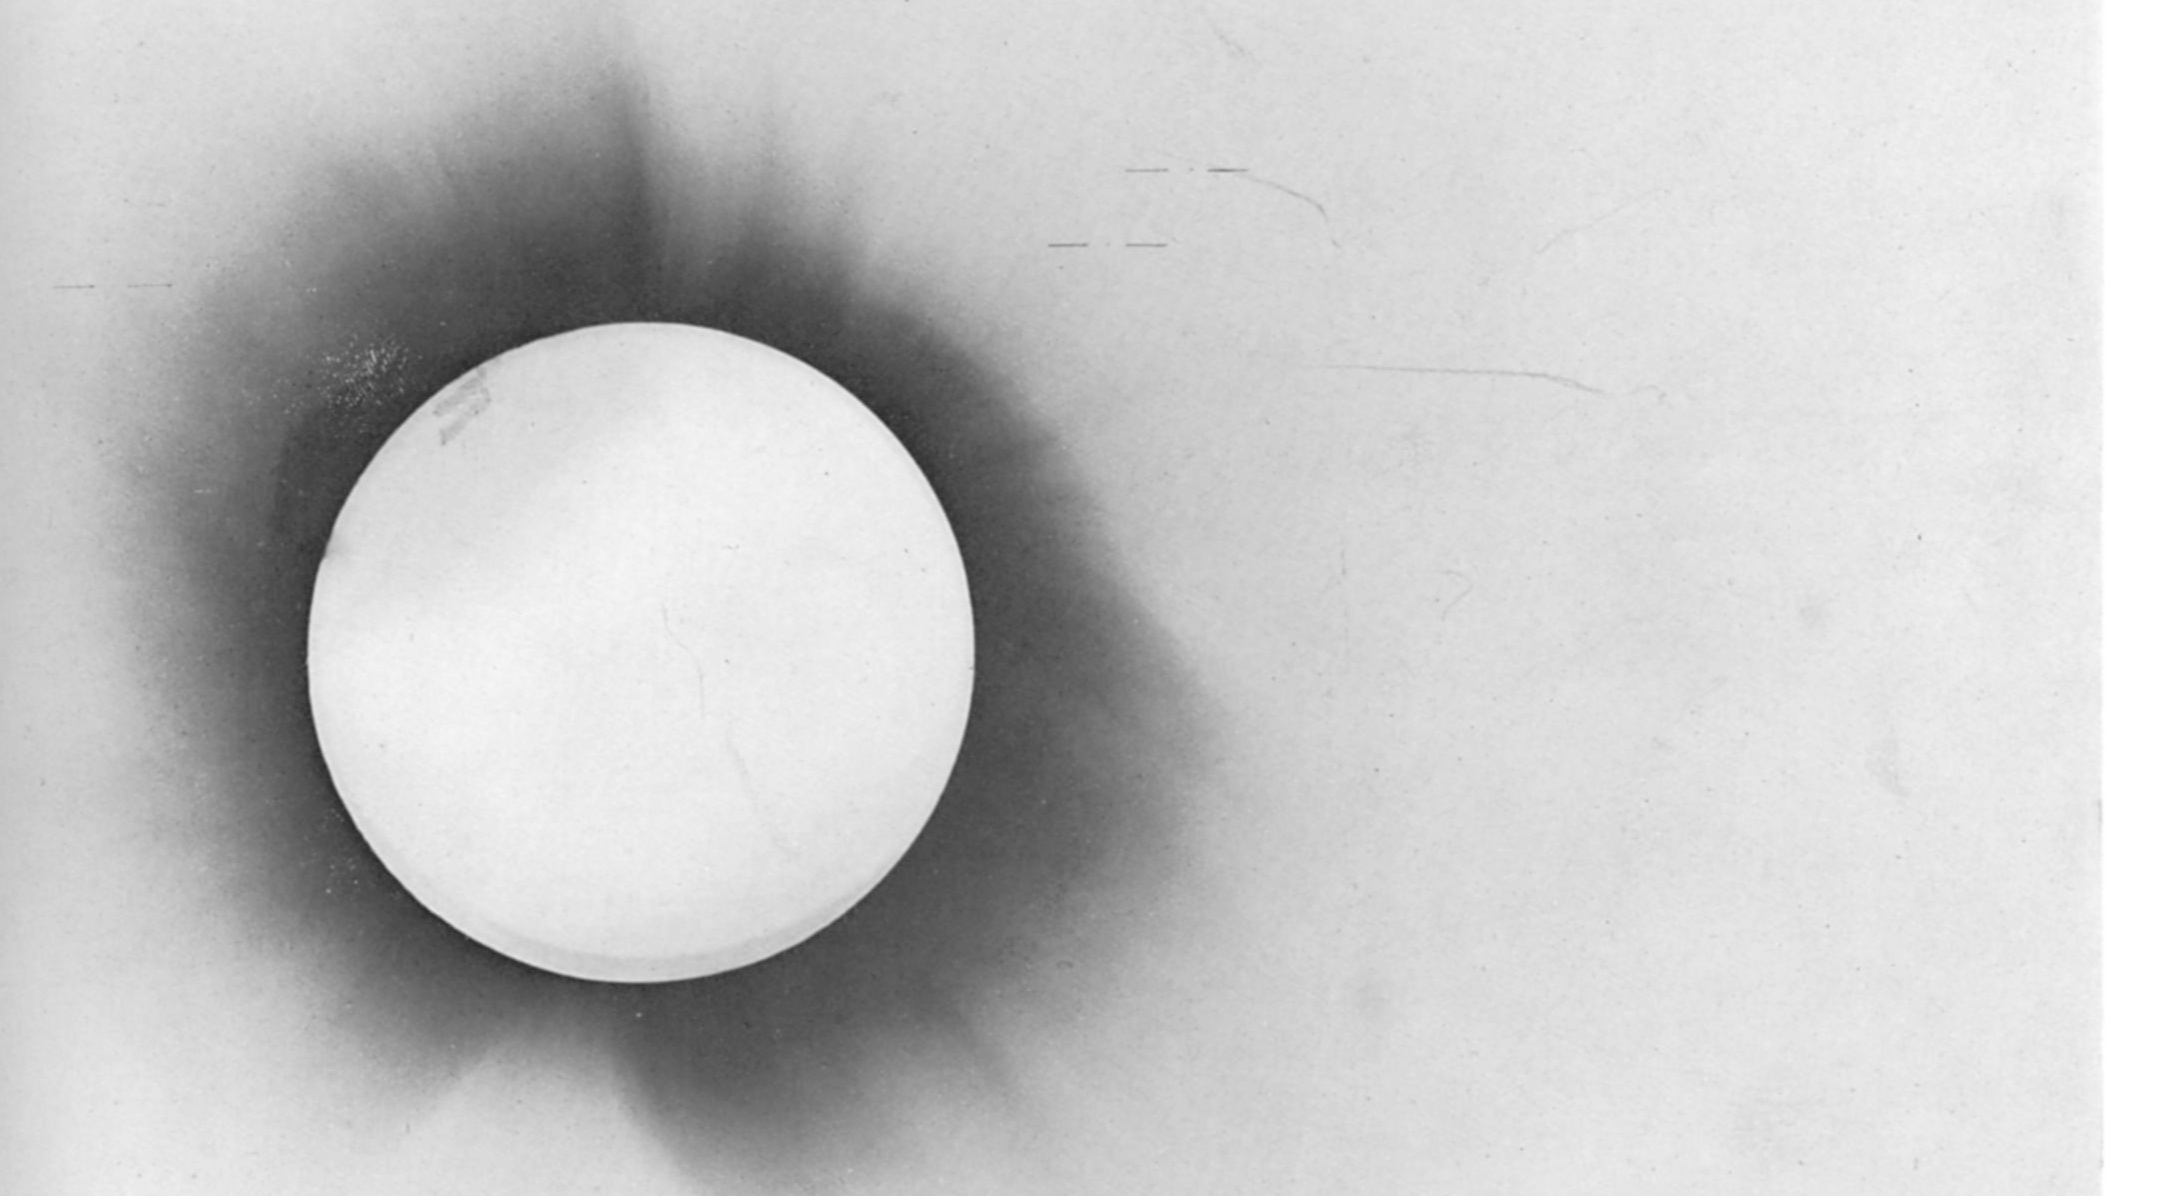
\includegraphics[width=\columnwidth]{Dyson.jpeg}
\caption{\label{fig:eclipse}Solar eclipse of 1919, which was studied to prove the bending of light by gravity. From \protect\citet{Dyson}.}
% It seems that you have to add the \protect command when putting citations inside Figure captions
% when using the MNRAS style package
\end{figure}

% figures should be put into the text as floats.
% Use the graphics or graphicx packages (distributed with LaTeX2e)
% and the \includegraphics macro defined in those packages.
% See the LaTeX Graphics Companion by Michel Goosens, Sebastian Rahtz,
% and Frank Mittelbach for instance.
%

\section{Structure of the report}

You are free to decide how best to present your work, but the following general structure should be used:

\begin{description}
\item[\textbf{Front matter}]	Title, registration number, date.

\item[\textbf{Abstract}]	The abstract should be up to about 200 words long and summarize the work and its conclusions. 

\item[\textbf{Introduction}]	The introduction should describe the project aims and give an overview of the background to the research topic, explaining what other people have done before you. 

\item[\textbf{Main body}] The main body of the report should begin with a discussion of any methods, theories, etc. relevant to the conduct of the project. You should then comment on your project plan. The results obtained and your analysis of them follows next. In some projects, it might be appropriate to summarize the key findings in a table. The final part is to discuss the results, putting them in their context and highlighting their significance. The structure will thus typically be as follows:
\begin{description}
% MNRAS doesn't like bullet lists. Here's my hack to get one.
\item[$\bullet$] methodology / experimental techniques;
\item[$\bullet$] discussion of any variations from your project plan submitted with your semester I report;
\item[$\bullet$] results, and their analysis;
\item[$\bullet$] critical discussion of results.
\end{description}

\item[\textbf{Conclusion}]	The report should end with a conclusion that summarizes the results obtained, places the work in its proper context and, if appropriate, makes suggestions for further related work. 

\item[\textbf{References}]	A reference list should be included for all works that are cited in the report. See Section~\ref{sec:refs}.

\item[\textbf{Appendices}]	Appendix A should be the project plan from your semester I report. Appendix B should be a statement about the effects of the industrial action and coronavirus on your project. Other appendices (e.g. computer source code, additional experimental results) should then be labelled consecutively with letters starting at \ref{other appendices}. 
\end{description}

\section{Report format}
\label{sec:format}

The report should be submitted in one of two formats:
\begin{itemize}
% It seems that nested bullet lists do work in MNRAS
\item Astrophysics projects should be submitted in the format of a paper in the \textit{Monthly Notices of the Royal Astronomical Society}.
\item All other reports should be submitted in the format of a paper in one of the \textit{Physical Review} Journals. You should choose the one that is most appropriate to your branch of physics:
\begin{itemize}
\item \textit{Physical Review A} for atomic, molecular, and optical physics, and quantum information;
\item \textit{Physical Review B} for condensed matter and materials physics;
\item \textit{Physical Review C} for nuclear physics;
\item \textit{Physical Review D} for particles, fields, gravitation, and cosmology;
\item \textit{Physical Review E} for statistical, nonlinear, biological, and soft matter physics.
\end{itemize}
\end{itemize}
If you are in any doubt about which of the \textit{Physical Review} formats to use, please ask your supervisor. The formats are, in fact, very similar, and you will not be penalized if you submit in the ``wrong''  \textit{Physical Review}  journal type.


The reports should be prepared following the instructions given on the journals' www sites.
\begin{itemize}
% Strange. The bullets are appearing now. I don't get this MNRAS package.
\item For \textit{Monthly Notices}, please see \url{https://academic.oup.com/mnras/pages/General_Instructions}.
\item For \textit{Physical Review} instructions, please see: \url{https://journals.aps.org/authors}.
\end{itemize}
The easiest way to get the right format is to use the \LaTeX\  files provided by the Journal.
\begin{itemize}
\item For \textit{Monthly Notices}, please see Section~2.1 of \url{https://academic.oup.com/mnras/pages/General_Instructions}. 
\item For \textit{Physical Review}, you  will need to use the REV\TeX~4.2 package. Information about how to get the REV\TeX~4.2 package is available at \url{http://journals.aps.org/revtex/}.
\end{itemize}
 If you do use these \LaTeX\ files, your report will automatically be set in the right format. Hence we strongly recommend using \LaTeX\ for your report.
 
 Some students may be unfamiliar with  \LaTeX\ and prefer to use a word-processor like WORD to prepare the report. This approach is acceptable, but the Journals only provide \LaTeX\ templates, and you will have to fiddle around to make your report have the right format. Download a recent paper from the appropriate journal, and reproduce it using your word processor. It is not necessary to reproduce the journal-specific headers and footers, and you will not be penalized if your report is not exactly in the right format, provided it looks like a good approximation to a pre-print paper in the relevant journal, as in this template. 








\section{References}
\label{sec:refs}


 You will need to cite the key papers that underpin your research in the introduction. You may need to give the references that explain the methodology that you are using, and you should  compare your own results to those that are published in the literature.

In giving the references, you should use standard scientific style, providing the following information: 
\begin{itemize}
\item author(s);
\item title of paper;
\item journal name, volume number, pages (or article ID number), year.
\end{itemize}
See \citet{Dyson} or  \citet{Einstein} for examples. If you cite books \citep{good book} or longer review articles, you should give the specific section of the book to which you are referring. 

% As far as I can see, you use \citet when the reference forms part of the sentence, 
% and \citep when it is not.

The references should be numbered for \textit{Physical Review} style, or follow the Harvard (name, date) system for  \textit{Monthly Notices} format (as in this report template). LaTeX users might find it helpful to use BibTeX \citep{BibteX}, while WORD users might want to consider using EndNote \citep{Endnote}.
If you are uncertain about any aspects of referencing, please look up the on-line tutorials provided by the library and refer to the Departmental referencing style for Physics \& Astronomy \citep{Referencing}. 




\section{Submitting the report}

% Hard copy submissions are not possible in 2020
% The following text is kept for use next year.
%You should submit \textbf{three} printed copies of your report together with your lab-book by Friday of week 12 of the Second Semester. Your printed reports should be mounted in the plastic binders that can be collected from F10.  
%The electronic version of your report should be submitted at the same time as the printed copies.

You should submit your report electronically using the Turnitin anti-plagiarism portal of PHY480 by \textbf{Friday of week 12 of Semester~II} (29th May). Please name your file: ``XXXXXXXXX-PHY480-report'', where ``XXXXXXXXX'' is your registration number. You should make sure that you comply stringently with the University's plagiarism guidelines \citep{plagiarism}. Note that minor changes to the original wording do not constitute a defence against accusations of plagiarism. If you are uncertain about any aspects of  plagiarism, please look up the on-line tutorials provided by the library \citep{Referencing}. 



%%%%%%%%%%%%%%%%%%%%%%%%%%%%%%%%%%%%%%%%%%%%%






% References
%
% The best way to enter references is to use BibTeX:

\bibliographystyle{mnras}
\bibliography{Sem2}


% Alternatively you could enter them by hand, like this:
% This method is tedious and prone to error if you have lots of references

%\begin{thebibliography}{99}
% The 99 argument allows you to have up to 99 references. If you have more than 99 (not recommended!), you will need to change it to 999.




%\end{thebibliography}


\appendix

\section{Semester One Project Plan}
\label{App:project plan}
\subsection{Postage Stamp Cutout}
Small 'postage stamp' cutouts from the large image are required to train SVMs. This requires that the previous source detection algorithm is functional. I believe this will take up to 10 hours. 
\subsection{Cross-Referencing Data}
After a satisfactory set of postage stamps is acquired, the cutouts need to be cross referenced with existing sky surveys to identify known objects to use as a training set. For now, the plan is to use SDSS to be the primary catalogue of reference. This should take up to 10 hours.
\subsection{PCA}
Performing a PCA on the data should be straightforwardly applying the algorithm. The issue is computing time, but I don't foresee this taking a vast amount of that either. I will allocate 5 hours to this for the time being.
\subsection{SVM and Kernal SVM}
Once the PCA is complete, a simple SVM can be performed, either using packaged algorithms or self-written ones. The limiting factor here is also computing time since an SVM algorithm is quite straight-forward to write.
Once that is complete, a kernal-SVM algorithm will be attempted. However since this is quite complex, a packaged solution will probably be used. I foresee many potential issues with trying this so I would allocate a total of 25 hours for this section.
\subsection{CNN}
After the SVM/PCA method is completed, a CNN will be attempted. Since the allure of a CNN is that it does not require the cutting out of postage stamps, that will be the first choice. However, it is still difficult to see how to properly make a training set for CNN this way. Further, many refinements would be necessary for a CNN, and training each iteration will be very time intensive. Therefore, I will conservatively estimate that 60 hours will be needed.
\subsection{Report}
After the project proper is finished, the report will be written. I expect some 10-20 hours will be spent on report writing.
\subsection{Other areas}
If there is any time to spare, other possible areas of work would be to make a Feedforward Neural Network and compare the results to kSVM. Otherwise, if the project proceeds vastly better than expected, an attempt to classify galaxies can be done.

\section{Effect of industrial action and coronavirus}
\label{2020 special}
The coronavirus epidemic meant that I traveled back to my home country of Hong Kong in late March. When I arrived, I was subject to 14 days of home quarantine with no broadband internet. However, this was mitigated somewhat by using mobile data, but was not idea. This also meant that project meetings needed to be scheduled at night time here, but this was by no means insurmountable. The coronavirus which also meant that the PhD student had pulled the GOTO data and placed it online is subsequently unavailable, hence only 32 GOTO images was used to train the data and exploring increasing the dataset was impossible. 


\section{Other stuff}
\label{other appendices}
You can have as many other appendices as you need. These appendices could contain, for example, computer source code, additional experimental results, lengthy tables of data, etc.  They could also contain material from your Semester~I report to which you wish to make reference. These appendices should be labelled consecutively with letters, starting at \ref{other appendices}.




% Don't change these lines
\bsp	% typesetting comment
\label{lastpage}
\end{document}

% End of mnras_template.tex













